\chapter{Elliptikus görbe kriptográfia}
\label{Chapter::ECC}

A fejezet célja, hogy bemutassa az Identity-based Encryption (IBE) megértéséhez szükséges matematikai hátteret. Ismerteti az elliptikus görbék matematikai elméletének felhasználását és szerepét a kriptográfiában. A fejezet elkészítéséhez Hankerson és munkatársai művét vettük alapul \citeyear{GuideToEllipticCurveCryptography}.

\section{Elliptikus görbék}

Az elliptikus görbékkel kapcsolatban rengeteg forrás létezik, hiszen már évszázadok óta tanulmányozzák matematikusok. Ahogyan azt Lang írta: \enquote{\textit{It is possible to write endlessly on Elliptic Curves (This is not a threat).}} \citeyear{Lang::EllipticCurve}. Ezzel szemben dolgozatunkban egy lényegre törő rövid áttekintést szeretnénk adni.
\\

Egy $\mathbb{F}$ test feletti elliptikus görbét azok a $P = (x, y) \in \mathbb{F}^2$ pontok alkotnak, amelyek kielégítik az alábbi egyenletet: $$y^2 + axy + by = x^3 + cx^2 + dx + e,$$ ahol $a, b, c, d, e, x, y \in \mathbb{F}$ és $a, b, c, d, e$ adottak. Az elliptikus görbék algebrai elméletéhez szükségünk van egy olyan képzetes, végtelen távoli $O$ pontra, amely rajta van minden függőleges egyenesen és az $x$-tengelyre vonatkozó tükörgépe önmaga, tehát $O = -O$.

A kriptográfiában kiemelt szereppel bírnak az úgynevezett Weierstrass elliptikus görbék \cite{Kobitz::ECC}, melyek egyenlete egyszerűbb az előbb látottnál: $$y^2 = x^3 + ax + b.$$ Egy ilyen görbéről látható példa a \dotref{Figure::ECC::EllipticCurve} ábrán. A dolgozat további részében is ilyen görbéket fogunk tekinteni.

\begin{figure}[H]
    \centering
    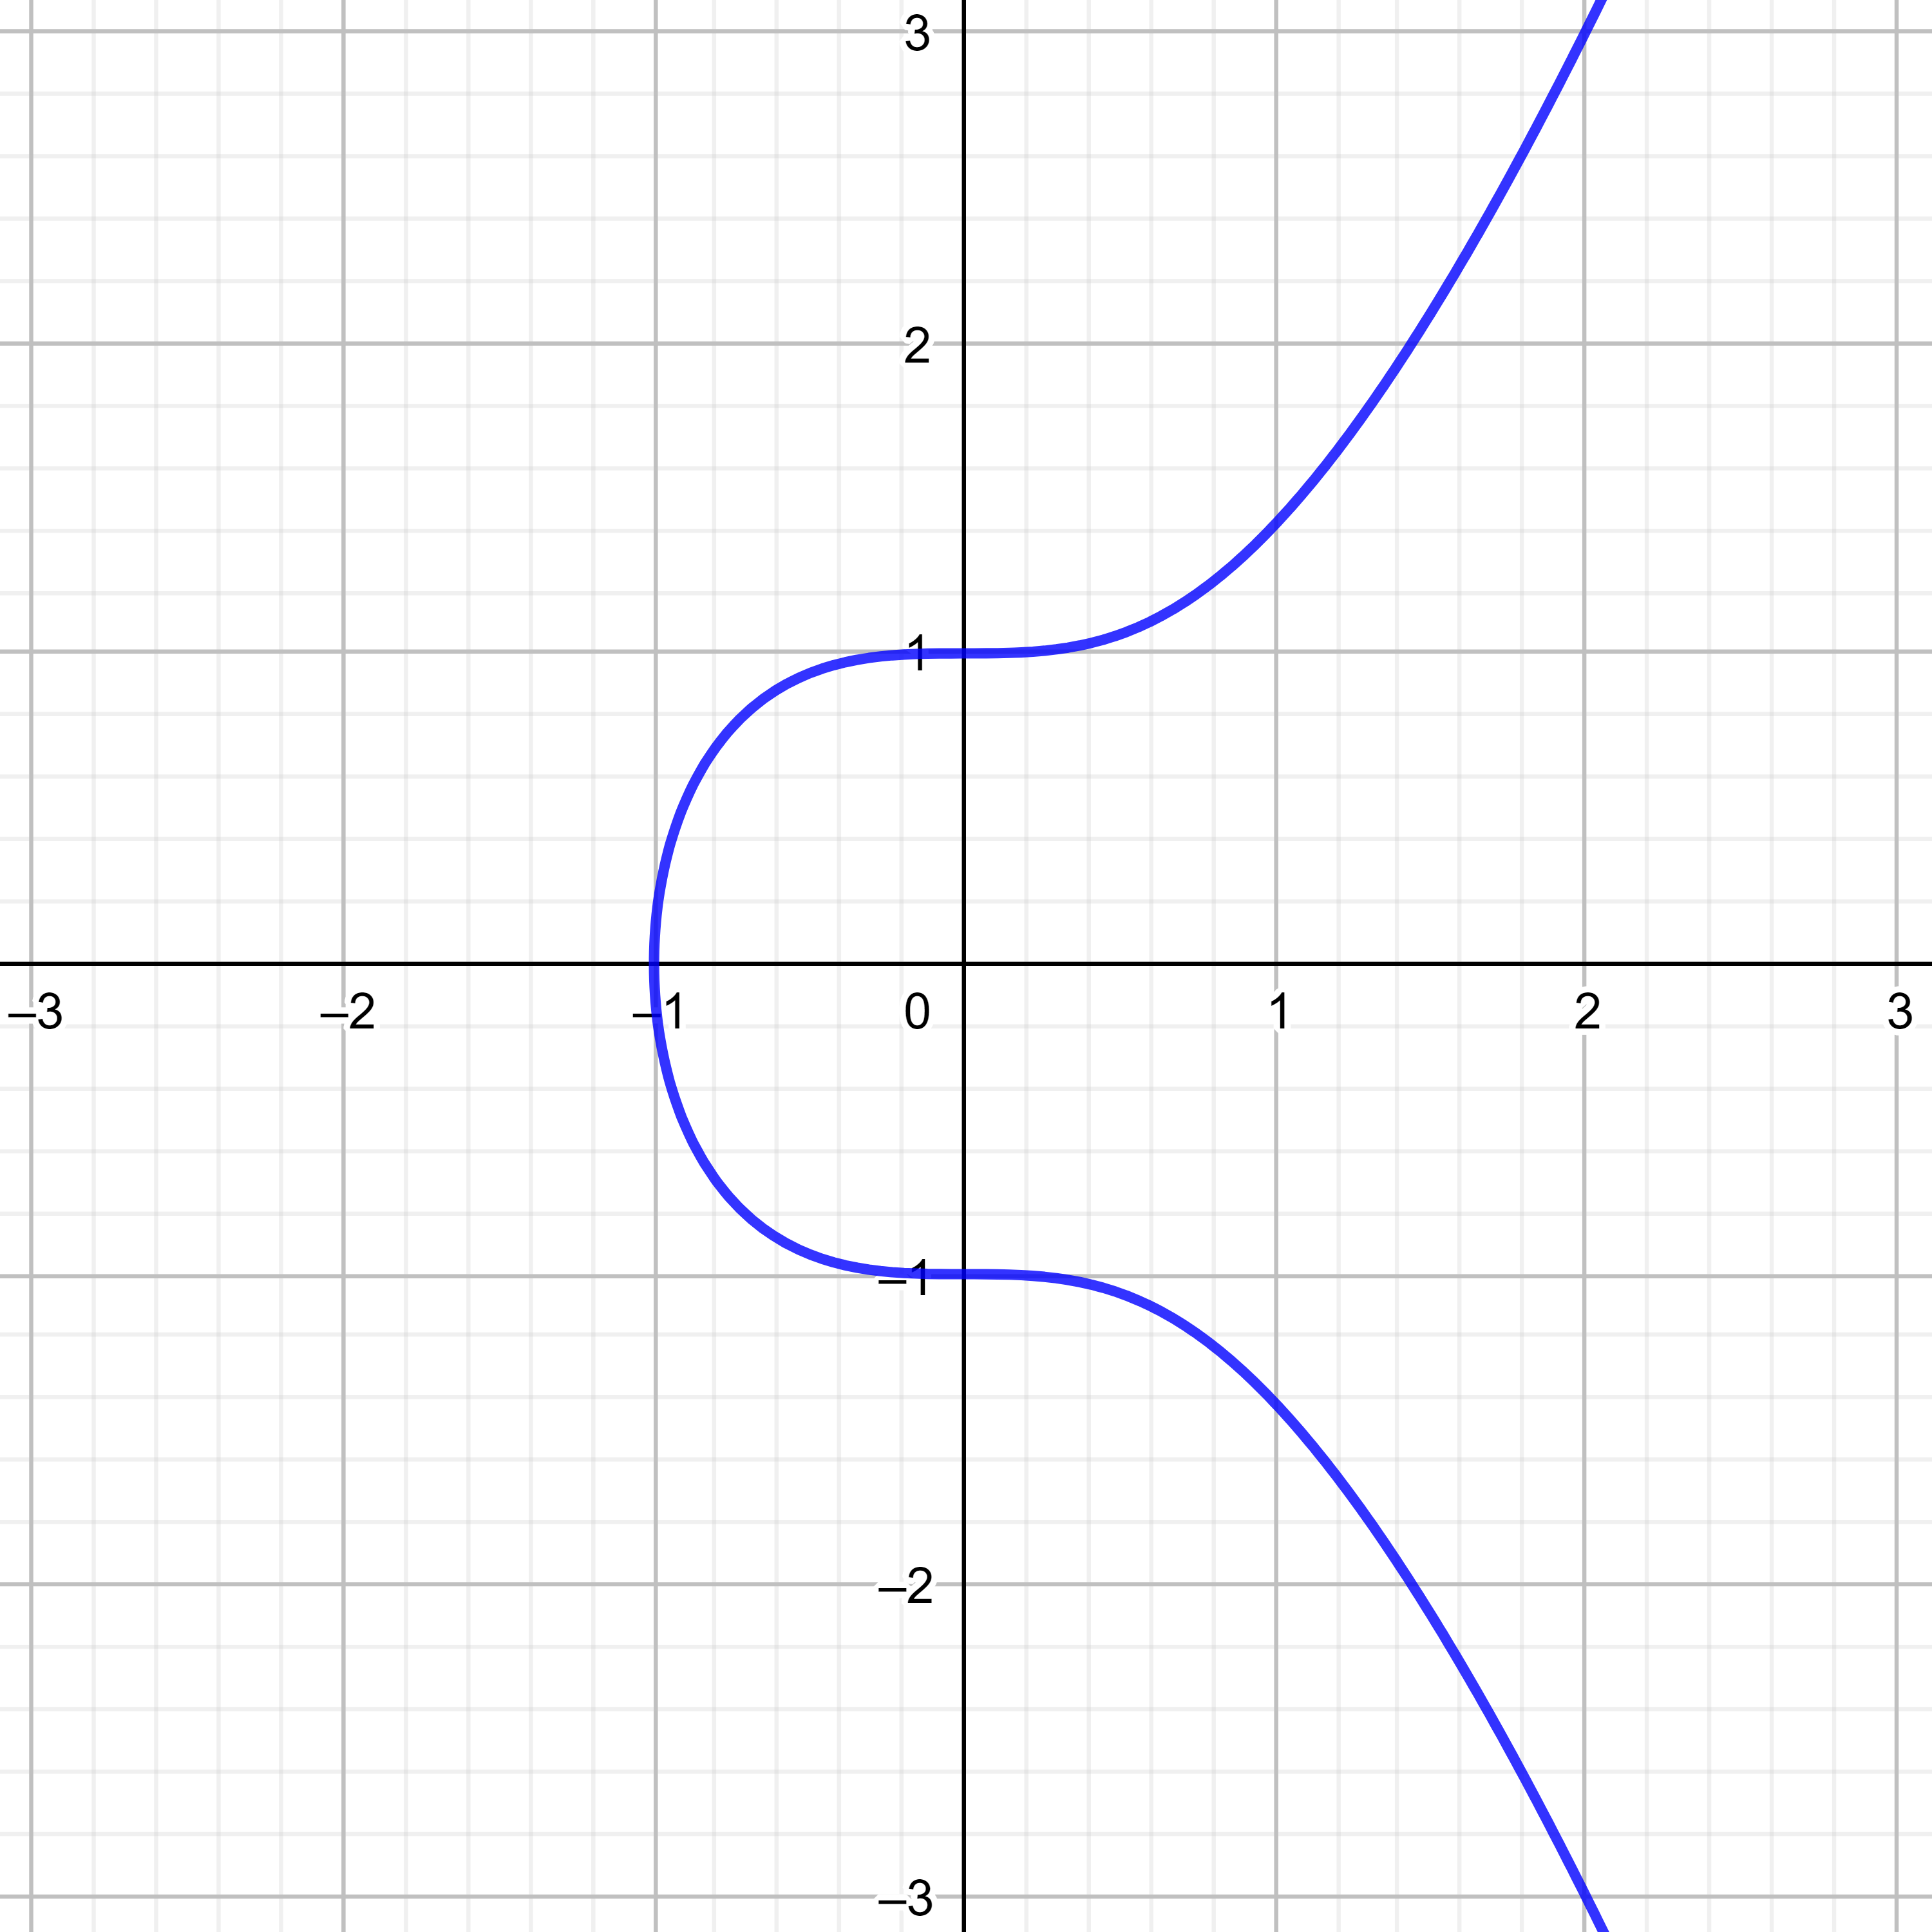
\includegraphics[width=0.4\textwidth]{02-elliptikus-gorbe-kriptografia/elliptikus-gorbe.png}
    \caption{Az $y^2 = x^3 + 1$ görbe a valós számok teste felett.}
    \label{Figure::ECC::EllipticCurve}
\end{figure}

\section{Műveletek elliptikus görbék pontjaival}

Az elliptikus görbék egy fontos tulajdonsága, hogy a görbe pontjai a megfelelően definiált összeadás művelettel Abel-csoportot alkotnak, amelyben az egységelem a korábban definiált $O$ végtelen távoli pont.

\subsection{Két pont összeadása}

Az összeadás szabályát geometriai úton a következőképp tekintjük. Legyen $E$ egy elliptikus görbe egy $K$ test felett, melynek jelölése $E(K)$. Legyen $P = (x_1, y_1)$ és $Q = (x_2, y_2)$ az $E$ elliptikus görbének két különböző pontja. Ekkor a $P$ és $Q$ pontok $R$ összegét a következő módon kapjuk.

Először húzzuk be a $P$-re és $Q$-ra illeszkedő egyenest. Ez az egyenes metszeni fogja az elliptikus görbét egy harmadik pontban. Ha ezt a harmadik pontot tükrözzük az $x$-tengelyre, akkor megkapjuk $R$-t. Adott pont önmagával vett összeadása (azaz duplázása) annyiban tér el az előzőtől, hogy egy olyan egyenest szükséges felrajzolni első lépésként, amely az elliptikus görbét az adott pontban érinti.

% Szándékosan van \ref és nem \dotref!
% A 2.2a és 2.2b után ugyanis nem kell pont.
Az előbbiekben leírt módszereket ábrázolják a \ref{Figure::ECC::EllipticCurveAddition1} és \ref{Figure::ECC::EllipticCurveAddition2} ábrák.

\begin{figure}[H]{}
    \centering
    \begin{subfigure}[t]{0.48\textwidth}
        \centering
        \captionsetup{width=.86\linewidth}
        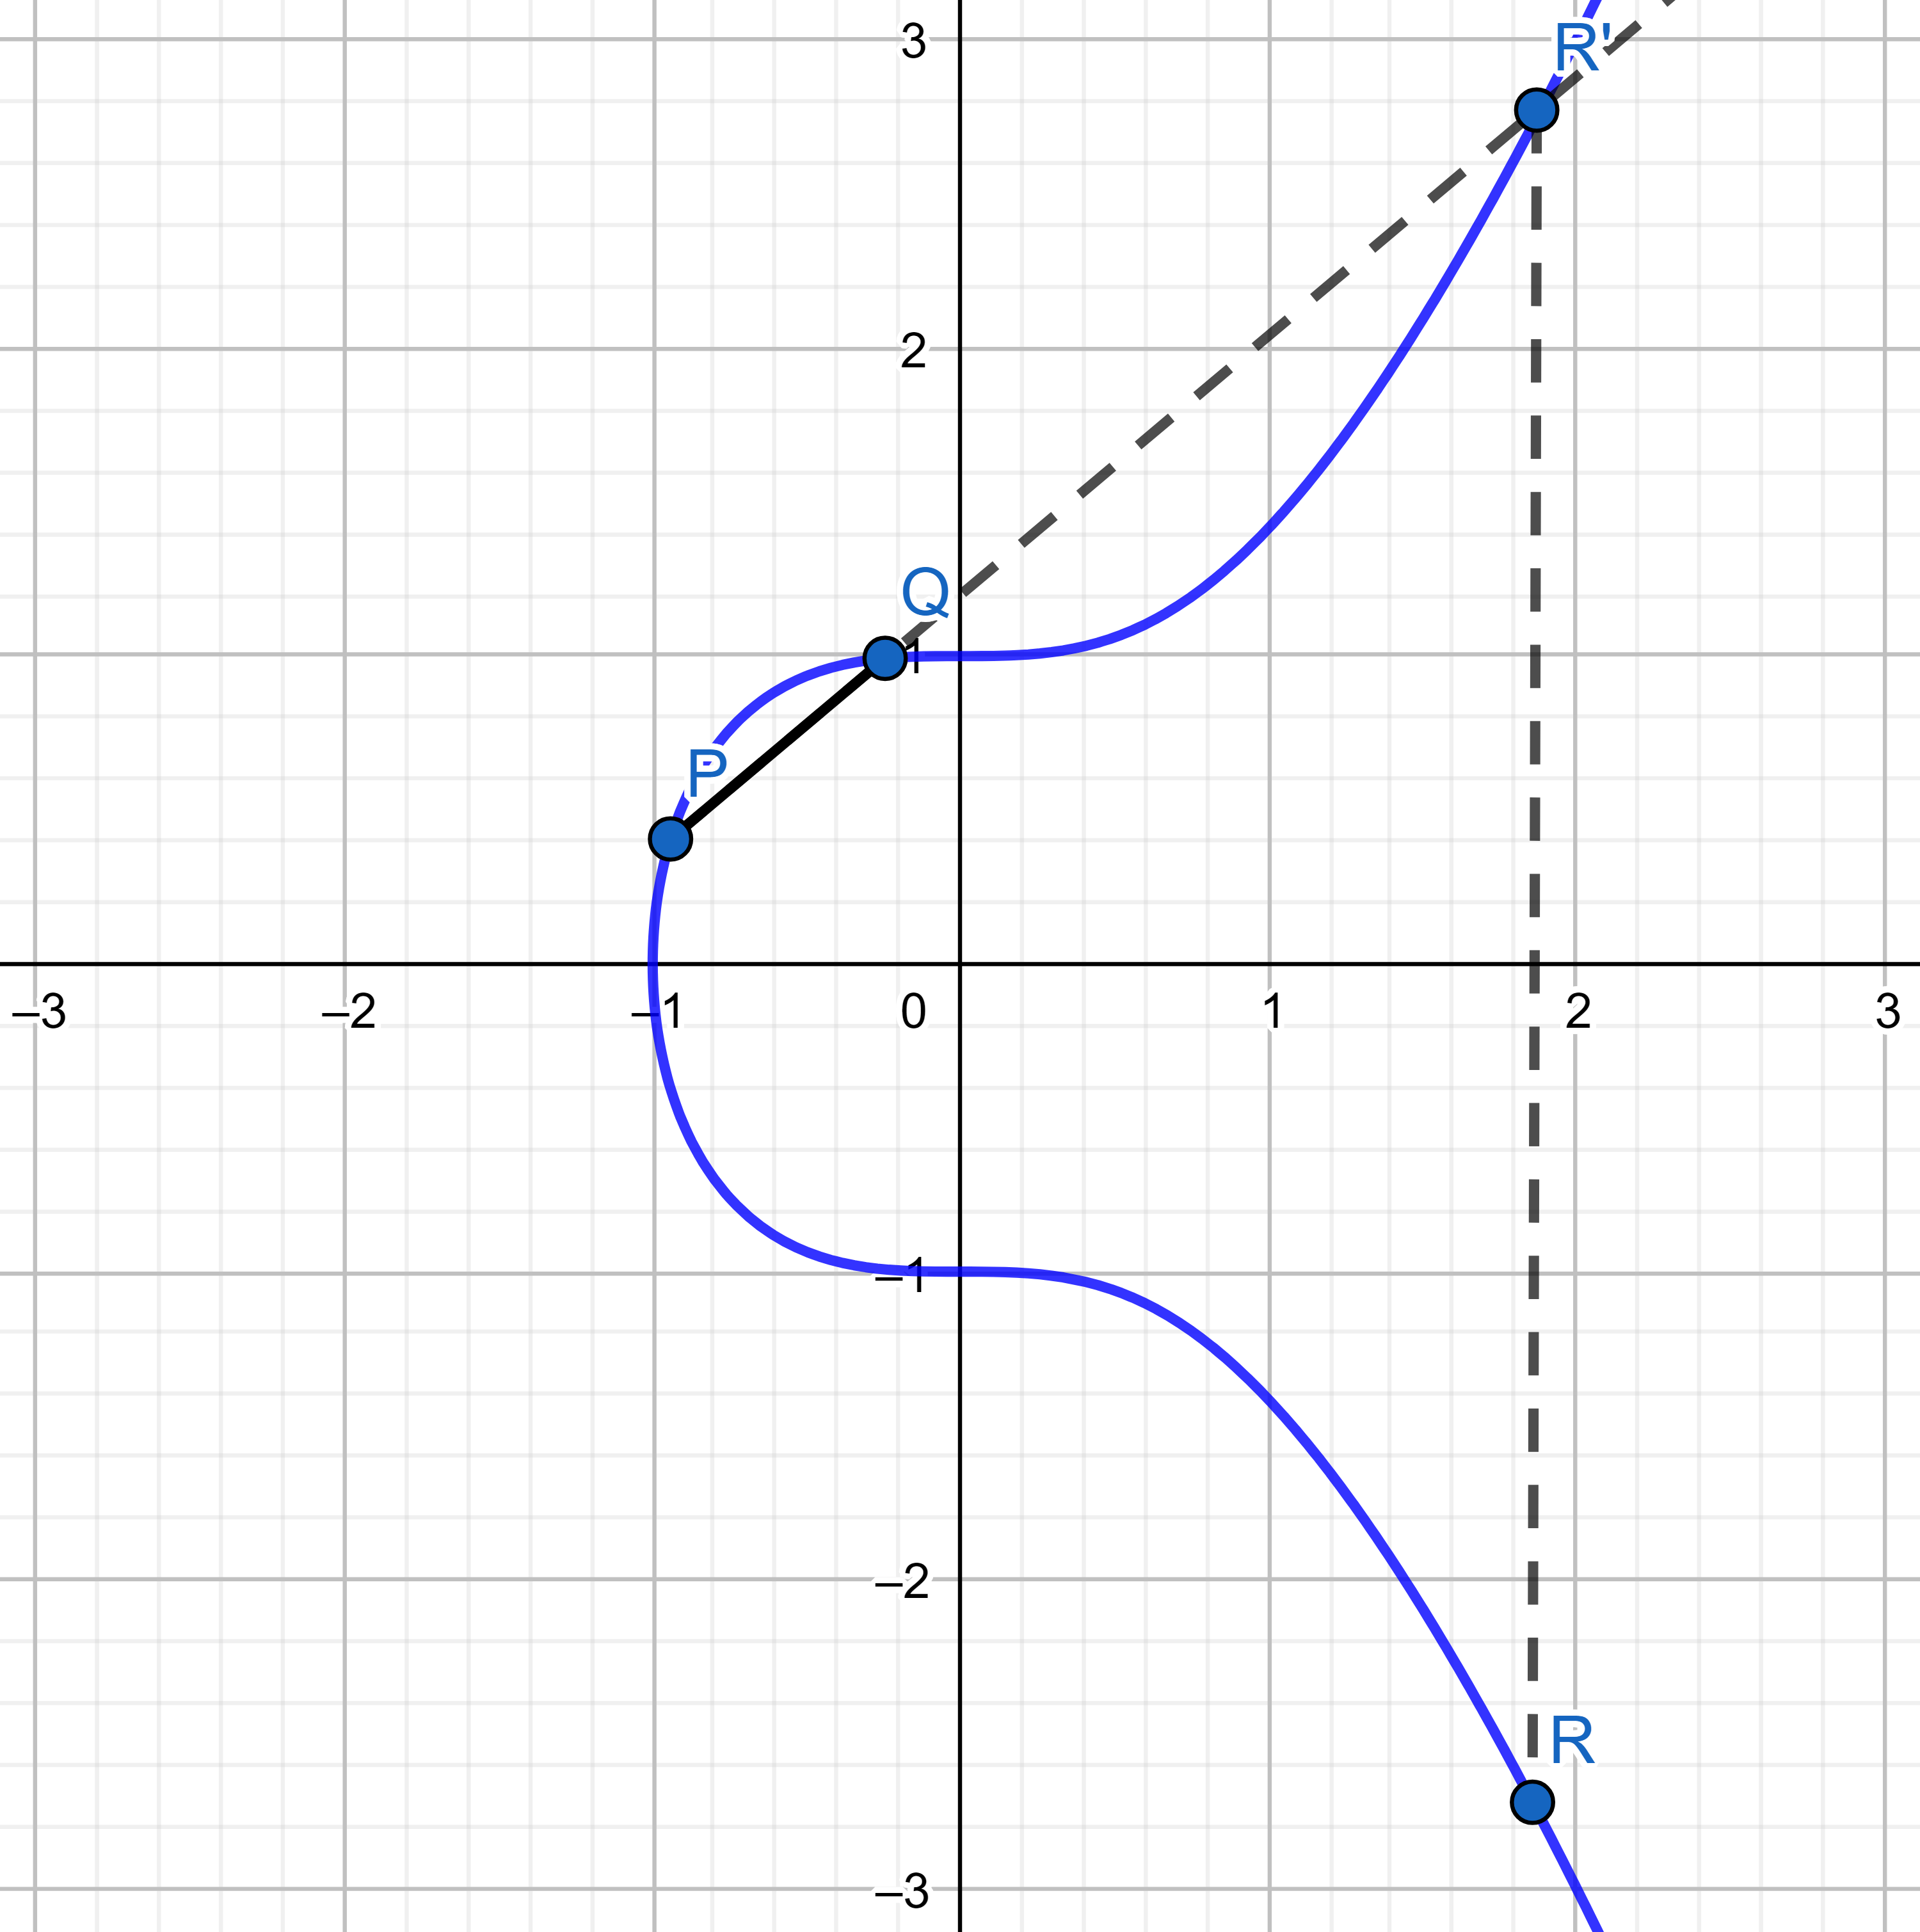
\includegraphics[width=.9\textwidth]{02-elliptikus-gorbe-kriptografia/elliptikus-gorbe-osszeadas1.png}
        \caption{Elliptikus görbe két különböző pontjának összeadása.}
        \label{Figure::ECC::EllipticCurveAddition1}
    \end{subfigure}
    \begin{subfigure}[t]{0.48\textwidth}
        \centering
        \captionsetup{width=.86\linewidth}
        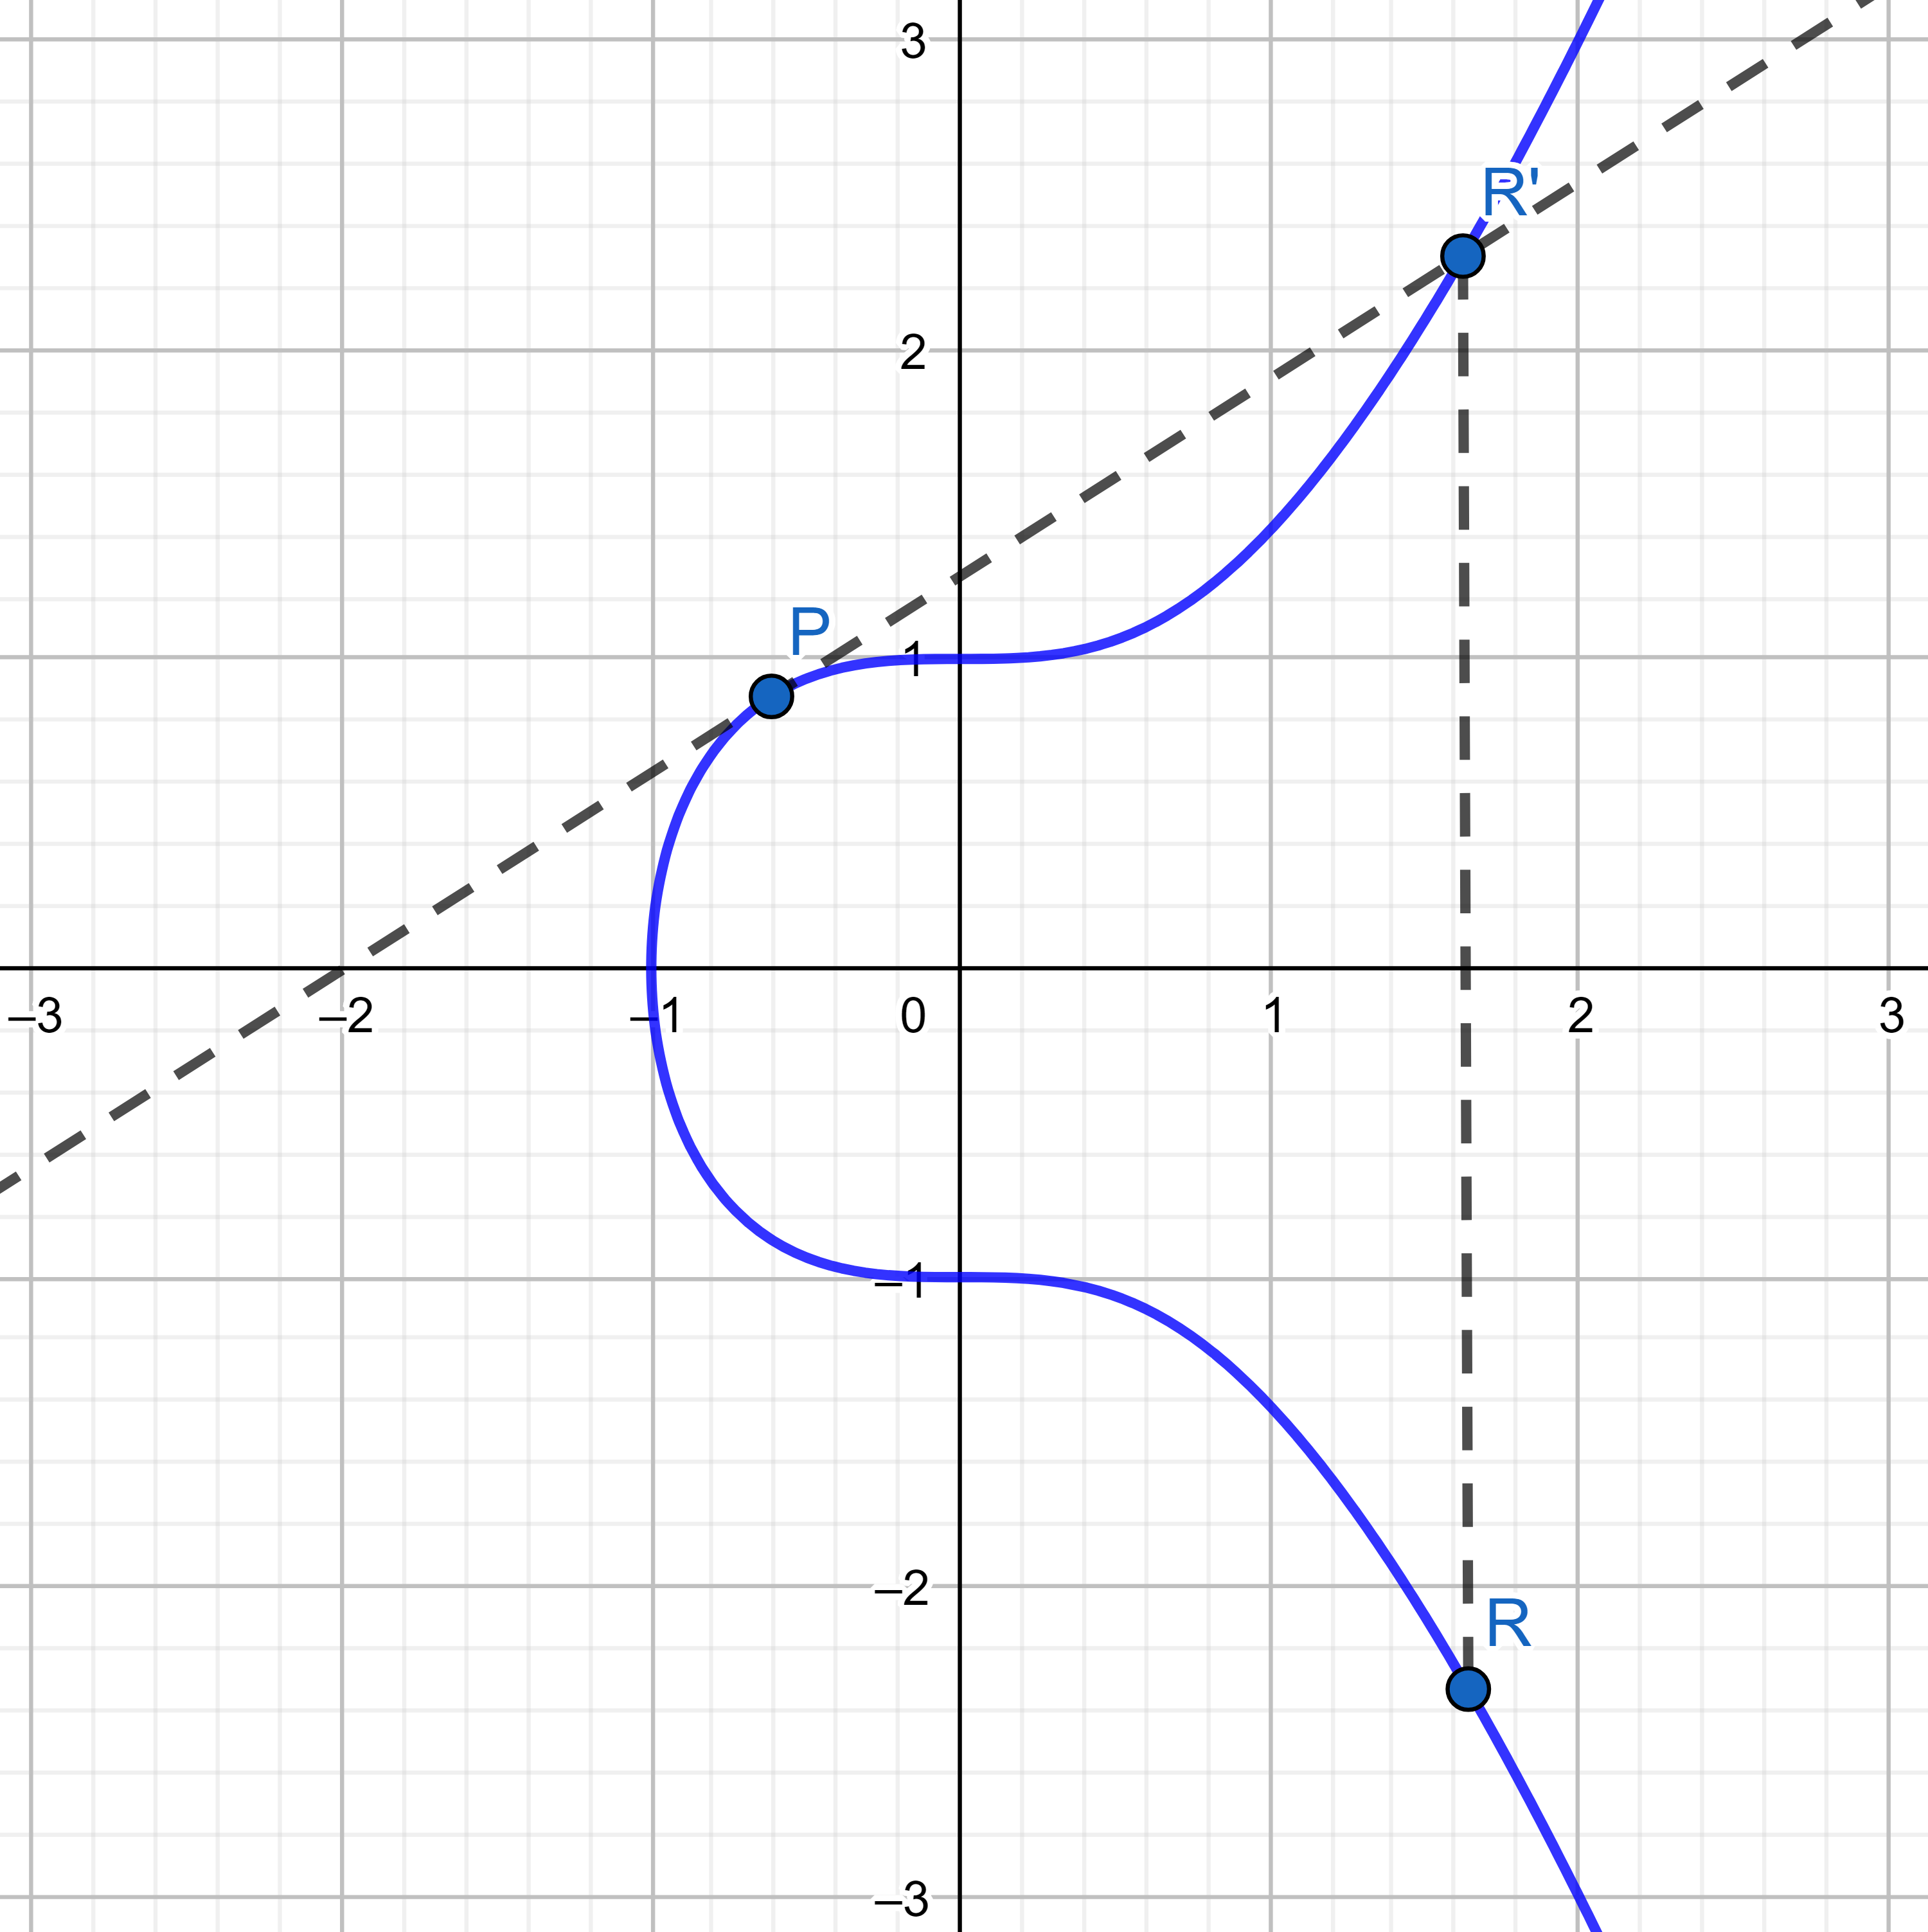
\includegraphics[width=.9\textwidth]{02-elliptikus-gorbe-kriptografia/elliptikus-gorbe-osszeadas2.png}
        \caption{Elliptikus görbe pontjának összeadása önmagával.}
        \label{Figure::ECC::EllipticCurveAddition2}
    \end{subfigure}
\end{figure}


\subsubsection{Az $E(K) : y^2 = x^3 + ax + b$ görbe tulajdonságai \protect\footnote{Ha $K$ karakterisztikája nem $2$.}}

\begin{outdentlist}
    \item[]
    \textbf{Egységelem.} $P + O = O + P = P$, minden $P \in E(K)$ esetén.

    \item[]
    \textbf{Ellentettek.} Ha $P = (x, y) \in E(K)$, akkor $(x, y) + (x, -y) = O$. Az $(x, -y)$ pontot $-P$-vel jelöljük és $P$ ellentettjének nevezzük. $-P$ is $E(K)$ egy pontja.

    \item[]
    \textbf{Pontok összeadása.} Legyen $P = (x_1, y_1) \in E(K)$ és $Q = (x_2, y_2) \in E(K)$, úgy hogy $P \neq \pm Q$. Ekkor $P + Q = (x_3, y_3)$, ahol 
    \begin{center}$x_3 = \big(\frac{y_2 - y_1}{x_2 - x_1}\big)^2 - x_1 - x_2$ és $y_3 = \frac{y_2 - y_1}{x_2 - x_1}(x_1 - x_3) - y_1$.\end{center}

    \item[]
    \textbf{Pont duplázás.} Legyen $P = (x_1, y_1) \in E(K)$, úgy hogy $P \neq -P$. Ekkor $2P = (x_3, y_3)$, ahol
    \begin{center}$x_3 = \big(\frac{3x_1^2 + a}{2y_1}\big)^2 - 2x_1$ és $y_3 = \frac{3x_1^2 + a}{2y_1}(x_1 - x_3) - y_1$.\end{center} Ha $P = -P$, akkor $2P = O$.
\end{outdentlist}

\subsection{Pontok skalár szorzása}

Az elliptikus görbe pontjait tetszőleges $k$ skalárral megszorozhatjuk, ami annyit jelent, hogy a pont $k$ példányát összeadjuk. Tehát ezen szorzás kiszámításának triviális módja az, ha elvégzünk $k - 1$ darab összeadást, azonban ez nagy $k$ esetén egy nagyon költséges lépéssorozat. Ezzel szemben létezik néhány kevésbé egyszerű, de sokkal hatékonyabb algoritmus is a szorzás elvégzésére.

\subsubsection{Double-and-Add}

A Horner séma \cite{Horner::HornerScheme} vagy \textit{Double-and-Add} nevű módszer egy hatékony megoldást nyújt elliptikus görbe pontjának skaláris szorzására, hasonlóan polinomok Horner-elrendezéséhez: Legyen a $k$ bináris felírása $\sum\limits_{i = 0}^{t-1} k_i 2^i$, ekkor $$kP = \sum_{i = 0}^{t-1} k_i 2^i(P) = k_0P + 2(k_1P + 2(k_2P + 2(... + 2(k_{t-1}P)...))).$$

A fenti képlet pszeudokódját az Algoritmus \dotref{algorithm:doubleAndAdd} jeleníti meg.
\begin{algorithm}[H]
    \floatname{algorithm}{Algoritmus}
    \caption{Double-and-Add algoritmus}
    \label{algorithm:doubleAndAdd}
    \begin{algorithmic}
        \Procedure{ScalarMultiply}{$k, P$} \Comment{$k=(k_{t-1},...,k_1,k_0)_2,P \in E(\mathbb{F}_q).$}
        \State $Q \gets O$
        \For {$i \gets t - 1$ downto $0$}
            \State {$Q \gets 2Q$}
            \If {$k_i = 1$} 
                \State $Q \gets Q + P$
            \EndIf
        \EndFor
        \State \Return {$Q$}
        \EndProcedure
    \end{algorithmic}
\end{algorithm}

Ezen felül számos lehetőség van optimalizálásra, mint például újabb, gyorsabb algoritmusok használata, azonban a dolgozat szemponjából ezek nem fontosak.

\section{Elliptikus görbék a kriptográfiában}

A kriptográfiában olyan elliptikus görbéket szokás alkalmazni, amelyek véges test felett vannak definiálva. A megelőzőleg bevezetett műveletek ekkor is érvényesek, az
eredmény pedig mindig a görbe egy pontja lesz. Elterjedtek az $\mathbb{F}_p$ felett értelmezett görbék, ahol $p$ egy prímszám. Ekkor a pontok koordinátáival mindig modulo $p$ kell számolni.

Az elliptikus görbén alapuló kriptográfiai sémák biztonságosságát az elliptikus diszkrét logaritmus probléma nehézsége adja.

\begin{definition*}
Az \textbf{elliptikus diszkrét logaritmus probléma} (ECDLP): Adott egy $E$ elliptikus görbe az $\mathbb{F}_q$ véges test felett, egy $n$ rendű $P \in E(\mathbb{F}_q)$ pont, valamint egy $Q$ pont, amely $P$ többszöröse. Keressük azt az $l \in [0, n - 1]$ egész számot, amelyre $Q = lP$ teljesül. Ezt a számot a $Q$ pont $P$ alapú elliptikus diszkrét logaritmusának nevezzük.
\end{definition*}

A definícióban bevezetett diszkrét logaritmus meghatározására nem ismert hatékony algoritmus.

\subsection{Miért válasszuk az elliptikus görbe kriptográfiát?}

Napjainkban az egyik legelterjedtebb aszimmetrikus titkosítási módszer az RSA algoritmus, ami a biztonságosságát a faktorizáció problémájából nyeri. Az RSA matematikai háttere sokkal egyszerűbbnek mondható, mint az elliptikus görbéken alapuló algoritmusoké, ezért implementálása sokkal egyszerűbb.

A faktorizáció ugyanakkor kevésbé nehéz probléma, mint az elliptikus diszkrét logaritmus probléma. Ahhoz, hogy az RSA algoritmus elérje a kellő biztonságosságot, sokkal nagyobb bithosszúságú kulcsokkal kell dolgoznia, mint az elliptikus görbéken alapuló algoritmusoknak \cite{Miller::ECC}. Ahogy a NIST ajánlásából olvasható, 160-521 bithosszúságú kulcs megfelelő az elliptikus görbén alapuló algoritmusok esetén \cite{NIST::EllipticCurve}, ezzel szemben az RSA esetén sokkal hosszabb, 1024-15360 bithosszúságú kulcsok szükségesek. Az NSA táblázat formájában is összevetette a NIST ajánlásait a különböző méretű AES kulcsok titkosításához szükséges RSA és elliptikus görbe kulcshosszakról \cite{NSA::EllipticCurve}.

A nagy kulcsok lassítják a számítást, ezért úgy gondoljuk, hosszú távon az elliptikus görbén alapuló algoritmusok jobban skálázhatók, mint az RSA.

\subsection{Elliptikus görbe könyvtárak}

Munkánk során több különböző elliptikus görbe aritmetikát megvalósító könyvtárat is megvizsgáltunk, amelyeket a \dotref{table::ECLibs} táblázat foglal össze.
\begin{table}[H]
    \centering
    \begin{tabular}{|l|l|l|}
        \hline
        \multicolumn{1}{|c|}{\textbf{Könyvtár neve}} & \multicolumn{1}{c|}{\textbf{Link}} & \multicolumn{1}{c|}{\textbf{Licenc}} \\ \hline
        libecc                                       & \url{https://github.com/ANSSI-FR/libecc} & BSD és GPL v2                         \\ \hline
        MIRACL                                       & \url{https://github.com/miracl/MIRACL}   & GNU AGPL v3                           \\ \hline
        PARI                                         & \url{https://pari.math.u-bordeaux.fr/}   & GNU GPL                               \\ \hline
        SageMath                                     & \url{http://www.sagemath.org/}           & GNU GPL                               \\ \hline
        snowshoe                                     & \url{https://github.com/catid/snowshoe}  & BSD 3-Clause                          \\ \hline
    \end{tabular}
    \caption{Elliptikus görbe aritmetikát megvalósító könyvtárak.}
    \label{table::ECLibs}
\end{table}
A libecc és a snowshoe dokumentációját elégtelennek találtuk, ami rendkívül megnehezítette volna a felhasználásukat.

A SageMath bár jól dokumentált, azonban egy óriási méretű könyvtár, melynek csak néhány elemére lett volna szükségünk. 

A PARI \cite{PARI} és a MIRACL között a döntést hozó tényező az volt, hogy a PARI fejlesztőit a témavezetőnk útján közelebbről is ismerjük.

Később azonban a fejlesztés során kellett rájönnünk, hogy céljaink elérése érdekében saját elliptikus görbe aritmetikát kell implementálnunk. 

Az egyik indok, ami erre a döntésre juttatott minket, hogy böngészőben kliensoldalon, akár mobil eszközökről is használhatóvá akartuk tenni a CryptID-nek nevezett könyvtárunkat, ami megköveteli a kis méretet az internetes adatforgalom csökkentése érdekében. A vizsgált elliptikus görbe műveleteket megvalósító könyvtárak számos olyan funkciót is tartalmaznak, amikre nekünk nem volt szükségünk, ezzel fölösleges mérettöbletet alkotva.

Másik fontos szempontunk az volt, hogy a saját implementációval úgy gondoljuk, leegyszerűsítettük a jövőbeli optimalizációs és kutatási tevékenységeink folytatását ezen a területen.
